% Relatório avulso da discussão dos contraexemplos A1-A6 (o mesmo texto entra no documento principal,
% biot_nao_saturado_agua_ar5.tex). Compilar com pdflatex duas vezes.
\documentclass[11pt,a4paper]{article}

\usepackage[T1]{fontenc}
\usepackage[utf8]{inputenc}
\usepackage{lmodern}
\usepackage{amsmath,amssymb}
\usepackage{geometry}
\usepackage{booktabs,array}
\usepackage{graphicx}
\usepackage{hyperref}
\geometry{margin=2.3cm}
\setlength{\parindent}{0pt}
\setlength{\parskip}{4pt}

\title{Contraexemplos a Rahardjo et al.\ (2007)\\
\large Discuss\~ao dos resultados: argumentos e verifica\c{c}\~ao}
\author{}
\date{29 de outubro de 2026}

\begin{document}
\maketitle
\vspace{-2em}

% Discussão dos contraexemplos A1-A6: argumentos levantados na análise dos resultados e cálculos mínimos para
% verificá-los. Incluída no documento principal (depois de secoes_literatura) e compilada sozinha em
% relatorio_discussao.tex; por isso não usa rótulos das outras seções.
%======================================================================
\section{Discuss\~ao dos contraexemplos: argumentos e verifica\c{c}\~ao}\label{sec:discussao}
%======================================================================

Esta se\c{c}\~ao registra a discuss\~ao dos resultados dos contraexemplos A1--A6 \`as conclus\~oes de Rahardjo et al.\
(2007): para cada item, o argumento levantado, o c\'alculo feito para verific\'a-lo e a conclus\~ao. Foram rodados
apenas os casos necess\'arios (Tabela~\ref{tab:disc_casos}); os demais argumentos foram verificados com os resultados
j\'a existentes.

\textbf{Defini\c{c}\~oes.} Talude de Rahardjo et al.: altura $H_s=10$~m, \^angulo $\alpha=45^\circ$, NA 5~m abaixo do
p\'e ($H_w=5$~m), chuva de 24~h, salvo indica\c{c}\~ao. Mohr--Coulomb com $c'=10$~kPa e $\phi'=26^\circ$
($\psi=\phi'/2=13^\circ$ no item A1), $\gamma=20$~kN/m$^3$; par\^ametro de Bishop $\chi=1$ salvo indica\c{c}\~ao;
suc\c{c}\~ao inicial hidrost\'atica limitada a 75~kPa. Solos $f_{10}$, $f_{50}$ e $f_{100}$: Fredlund--Xing com
$a=10$, 50 e 100~kPa ($n=m=1$) e $k_s=10^{-4}$, $10^{-5}$ e $10^{-6}$~m/s (360, 36 e 3,6~mm/h). \emph{Modelo do
artigo}: percola\c{c}\~ao desacoplada com $p_a=0$ (SEEP/W no artigo); \emph{modelo completo}: acoplado, com a fase de ar
ativa ($p_a=0$ s\'o na superf\'icie); $\psi$ \'e o \^angulo de dilat\^ancia; o FS \'e o da redu\c{c}\~ao de resist\^encia
(SRM). Os itens A1--A6, a S\'erie~B (FS m\'inimo em fun\c{c}\~ao da intensidade $I_r$) e os grupos do item A2 (G1: solo
$f_{100}$, $\alpha=63{,}4^\circ$, $H_s=10$~m) s\~ao os da se\c{c}\~ao de contraexemplos do documento principal.

\begin{table}[h!]
\centering\small
\caption{C\'alculos feitos para a discuss\~ao (todos com o programa \texttt{SlopeRainfall}; scripts
\texttt{contraexemplos.py}, itens A1c, A3c, A4c e A6, e \texttt{fase\_ar.py}, grupo G4).}\label{tab:disc_casos}
\begin{tabular}{llp{8.6cm}}
\toprule
item & casos & o que verifica\\
\midrule
A1c & 9 & intensidade cr\'itica (FS chega a 1): modelo completo com $\psi=0$ e $I_r=18$, 22, 26, 30, 33, 36 e 54~mm/h,
com $\psi=\phi'$ e 30~mm/h; modelo do artigo com 48~mm/h; FS de hora em hora; toler\^ancia do SRM 0,002\\
G4 (A2) & 3 & refinamento da malha no talude do G1, 36~mm/h, ar ativo: $h_{sup}=0{,}75$ (malha padr\~ao), 0,5 e
0,35~m; toler\^ancia 0,002\\
A3c & 2 & anisotropia no modelo completo ($\psi=\phi'$): isotr\'opico e $k_1$ paralelo \`a face ($\theta=135^\circ$),
90~mm/h; toler\^ancia 0,002\\
A4c & 2 & $\chi=S_e$ no lugar de $\chi=1$: $H_w=15$~m, 36~mm/h, suc\c{c}\~ao inicial limitada a 75 e 300~kPa;
toler\^ancia 0,01\\
A6 & 4 & mesmo volume (864~mm) em dura\c{c}\~oes em torno de $t^*=V/k_s$: $f_{10}$ com 0,75~h, $f_{100}$ com 240 e
480~h, e o $f_{10}$ com 3~h e passo de tempo 4 vezes menor (verifica\c{c}\~ao); toler\^ancia 0,01\\
\bottomrule
\end{tabular}
\end{table}

\subsection{Crit\'erio de ruptura e resolu\c{c}\~ao do FS}

Considera-se ruptura FS $\le1$. O FS de cada instante \'e calculado com as press\~oes daquele instante congeladas; um
valor abaixo de 1 n\~ao descreve um estado f\'isico, porque o talude j\'a teria se movido e redistribu\'ido as
press\~oes, e mede apenas quanto o equil\'ibrio foi ultrapassado. O que decide \'e se o FS chega a 1, com que chuva e
em que instante. O SRM devolve o \'ultimo fator de redu\c{c}\~ao que convergiu: o FS escrito \'e um limite inferior,
com erro menor que a toler\^ancia da bissec\c{c}\~ao (0,002 nos itens A1c, A3c e G4, op\c{c}\~ao \texttt{tolfs}; 0,01, o
padr\~ao do programa, nos c\'alculos anteriores e nos itens A4c e A6). Com a malha padr\~ao, o erro de
discretiza\c{c}\~ao acrescenta cerca de 0,01 (item A2); valores de 1,00 a cerca de 1,02 s\~ao tratados como
equil\'ibrio limite.

%----------------------------------------------------------------------
\subsection{A1: o que importa \'e a intensidade com que o FS chega a 1}

\textbf{Argumento.} Com o crit\'erio FS $\le1$, tanto faz se o patamar \'e 1,00 ou 0,84--0,85: nos dois casos o
talude j\'a rompeu, e um FS abaixo de 1 pode n\~ao ser f\'isico. O que importa \'e se, a partir de uma
intensidade-limite, o FS chega a 1 (ou menos) e se mant\'em nesse patamar; nesse sentido a afirma\c{c}\~ao do artigo
faz sentido, porque mesmo aumentando a intensidade o FS fica em 1 ou abaixo.

\textbf{Verifica\c{c}\~ao.} Intensidades intermedi\'arias no modelo completo com $\psi=0$ (18 a 54~mm/h) e com
$\psi=\phi'$ (30~mm/h), FS de hora em hora e toler\^ancia 0,002, e o modelo do artigo com 48~mm/h; com os casos do
item A1 ($\psi=0$, $\phi'/2$ e $\phi'$) e da variante desacoplada da S\'erie~B (Tabela~\ref{tab:disc_A1},
Fig.~\ref{fig:disc_A1}). Com $\psi<\phi'$ o FS do SRM \'e calculado com $\psi=\phi'$ (a redu\c{c}\~ao de
resist\^encia n\~ao associativa n\~ao converge); depois que o transiente perde o equil\'ibrio ($t_f$), ele segue com a
resist\^encia aumentada, s\'o para acompanhar as press\~oes.

\begin{table}[h!]
\centering\small
\caption{A1: FS m\'inimo (24~h de chuva, $f_{50}$) e intensidade cr\'itica $I_c$ (menor $I_r$ com FS m\'inimo
$\le1{,}01$, por interpola\c{c}\~ao linear). $t_f$: instante em que o transiente perde o equil\'ibrio (s\'o com
$\psi=0$). Em it\'alico, toler\^ancia do SRM 0,01 (item A1 e S\'erie~B).}\label{tab:disc_A1}
\setlength{\tabcolsep}{4pt}
\begin{tabular}{lccccccccc}
\toprule
$I_r$ (mm/h) & 18 & 22 & 26 & 30 & 33 & 36 & 48 & 54 & $I_c$ (mm/h)\\
\midrule
completo, $\psi=0$ & 1,316 & 1,148 & 1,003 & 0,978 & 0,971 & 0,968 & & 0,963 & 25,8\\
\quad $t_f$ (h) & -- & -- & 21,5 & 18 & 16,8 & 15,5 & & 12,5 &\\
completo, $\psi=\phi'/2$ & \emph{1,319} & & & & & \emph{1,005} & & \emph{1,004} & $\le36$\\
completo, $\psi=\phi'$ & \emph{1,319} & & & 1,011 & & \emph{1,003} & & \emph{1,000} & 31,1\\
artigo & \emph{1,609} & & & & & \emph{1,176} & 1,010 & \emph{0,966} & 48,0\\
\bottomrule
\end{tabular}
\end{table}

\begin{figure}[h!]
\centering
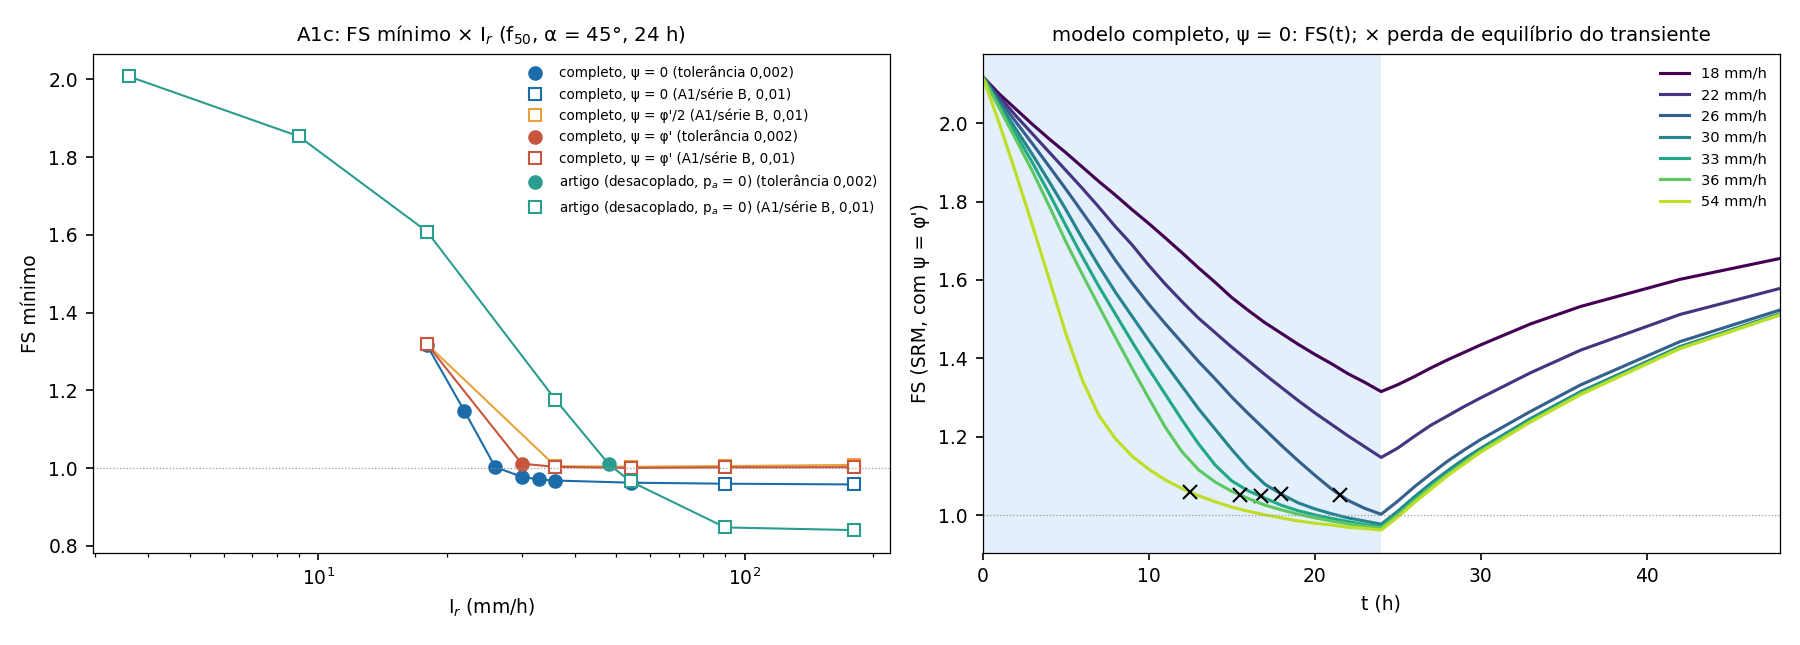
\includegraphics[width=\textwidth]{figuras/contra_A1_criterio.png}
\caption{A1: FS m\'inimo $\times$ $I_r$ nos quatro modelos (cheio: toler\^ancia 0,002; vazio: 0,01) e FS($t$) do
modelo completo com $\psi=0$ (o FS do SRM \'e calculado com $\psi=\phi'$; $\times$: perda de equil\'ibrio do
transiente com $\psi=0$).}\label{fig:disc_A1}
\end{figure}

\textbf{Conclus\~ao.} Concorda-se com o crit\'erio, e com ele a leitura do item A1 muda. Todos os modelos t\^em uma
intensidade cr\'itica $I_c$, a partir da qual o FS chega a 1 durante a chuva e n\~ao volta a subir enquanto chove
(Fig.~\ref{fig:disc_A1}, \`a direita, para $\psi=0$; Tabela~\ref{tab:disc_A1} para os demais): nesse sentido a
afirma\c{c}\~ao do artigo se mant\'em. O que muda \'e o valor. Com o mesmo n\'ivel (FS $\le1{,}01$), $I_c\approx48$~mm/h
na reprodu\c{c}\~ao do modelo do artigo, 31~mm/h no modelo completo com $\psi=\phi'$ e 26~mm/h com $\psi=0$, isto \'e,
$1{,}3k_s$, $0{,}9k_s$ e $0{,}7k_s$: as hip\'oteses do artigo superestimam em 55 a 86\% a chuva que rompe o talude
(contra a curva publicada, Eq.~6, que d\'a FS $=1$ com 40~mm/h, em 28 a 54\%). Nas chuvas fortes elas tamb\'em atrasam a
ruptura: com 54, 90 e 180~mm/h o FS do modelo do artigo chega a 1 \`as 22,8, 20,1 e 19,3~h, contra 1,01 \`as 17,9, 18,3
e 17,2~h no modelo completo com $\psi=\phi'$ e a perda de equil\'ibrio \`as 12,5, 12 e 11,75~h com $\psi=0$ (2 a 5~h e
8 a 10~h de atraso). A dilat\^ancia n\~ao decide se h\'a intensidade cr\'itica, mas a desloca em cerca de 20\% (de 26
para 31~mm/h), antecipa a ruptura em cerca de 6~h e decide o que acontece depois: com $\psi=0$ o transiente perde o
equil\'ibrio (entre 21,5~h com 26~mm/h e 11,75~h com 180~mm/h; com 22~mm/h n\~ao perde); com $\psi=\phi'/2$ ou $\phi'$ o
FS para em 1,000--1,011, em equil\'ibrio limite com deforma\c{c}\~ao pl\'astica. Com $\psi=0$ a perda de equil\'ibrio
vem quando o FS do SRM, calculado com $\psi=\phi'$, ainda vale 1,05 a 1,06: o SRM associativo superestima em cerca de
5\% o FS de um solo sem dilat\^ancia, ou parte da perda de equil\'ibrio \'e num\'erica, o que estes c\'alculos n\~ao
separam. Por isso, com $\psi=0$, o instante da ruptura \'e $t_f$ e $22<I_c\le26$~mm/h; os FS abaixo de 1 dessa linha
usam press\~oes do transiente seguido com a resist\^encia aumentada. O valor do patamar abaixo de 1 (0,96 ou
0,84--0,85) n\~ao distingue taludes que j\'a romperam; o patamar s\'o importa quando fica acima de 1, como no item A3
com $k_1$ horizontal (1,05), em que nenhuma chuva de 24~h, at\'e 360~mm/h, leva o FS a 1. A grandeza a comparar entre
modelos \'e, portanto, $I_c$ e o instante da ruptura, n\~ao o FS m\'inimo.

%----------------------------------------------------------------------
\subsection{A2: ar aprisionado e a margem de 1\%}

\textbf{Argumento.} Em solos pouco perme\'aveis o ar pode ficar retido em bols\~oes, sem escapar pela superf\'icie,
reduzindo a suc\c{c}\~ao e a resist\^encia ao cisalhamento; por isso o FS fica abaixo do calculado com ar passivo. No
exemplo, com ar ativo o FS chega a 1,01, o que pode ser ruptura: o FS cai quando a malha \'e refinada, e 1\% \'e muito
pouco.

\textbf{Verifica\c{c}\~ao.} O mecanismo foi verificado nos campos de press\~ao j\'a calculados do G1 com 36~mm/h
(m\'edias por faixa de profundidade \`as 24~h) e nos tempos de alagamento. A margem foi verificada refinando a malha do
G1 com 36~mm/h e ar ativo, com toler\^ancia 0,002 (Tabela~\ref{tab:disc_A2}).

\begin{table}[h!]
\centering\small
\caption{A2: FS do G1 com ar ativo e 36~mm/h em tr\^es malhas; $h_{sup}$ \'e o tamanho dos elementos at\'e 2~m de
profundidade (o tamanho m\'aximo no interior diminui na mesma propor\c{c}\~ao). Toler\^ancia do SRM 0,002.}
\label{tab:disc_A2}
\begin{tabular}{lccc}
\toprule
$h_{sup}$ (m) & 0,75 (padr\~ao) & 0,5 & 0,35\\
tri\^angulos & 1620 & 3597 & 7314\\
\midrule
FS inicial & 1,775 & 1,761 & 1,752\\
FS m\'inimo (24~h) & 1,0154 & 1,0122 & 1,0090\\
$p_a$ m\'axima (kPa) & 37,9 & 38,0 & 38,2\\
volume infiltrado em 24~h (m$^3$/m) & 11,5 & 11,1 & 10,9\\
\bottomrule
\end{tabular}
\end{table}

\textbf{Conclus\~ao.} O mecanismo confere, com duas ressalvas. Primeira: no modelo n\~ao s\~ao bols\~oes isolados. Com
a base e as laterais fechadas ao ar e a chuva sobre toda a superf\'icie, o ar de toda a zona n\~ao saturada entre a
frente de umedecimento e o NA fica preso e \'e comprimido pela \'agua que entra; \'e o cen\'ario de aprisionamento
m\'aximo, que n\~ao exclui bols\~oes em situa\c{c}\~oes menos confinadas. A press\~ao n\~ao \'e uniforme: \`as 24~h, $p_a$
vale em m\'edia 32~kPa entre 0,5 e 5~m de profundidade e 24~kPa entre 5 e 8~m ($p_a$ m\'axima de 36 a 38~kPa nos casos
do G1). Segunda: a suc\c{c}\~ao n\~ao cai. Entre 2 e 5~m de profundidade, com ar ativo, $p_a-p_w=38$~kPa, contra 24~kPa
com ar passivo, porque entra menos \'agua (10,4 a 11,6 contra 13,5 a 17,9~m$^3$/m em 24~h); o que sobe \'e $p_w$ ($-6$
contra $-24$~kPa), empurrada pelo ar comprimido. Com $\chi=1$ a tens\~ao efetiva depende s\'o de $p_w$ e cai; com
$\chi<1$ a press\~ao m\'edia nos poros, $\chi p_w+(1-\chi)p_a$, acompanha tamb\'em $p_a$. Por isso o FS fica abaixo do
calculado com ar passivo mesmo com menos \'agua. A baixa permeabilidade importa porque a superf\'icie alaga e o ar s\'o
sai por ela; o pr\'oprio ar antecipa o alagamento (com 9~mm/h, o primeiro v\'ertice alaga \`as 6~h com ar ativo e \`as
11,75~h com ar passivo, e \`as 24~h est\~ao alagados 83 contra 41 dos 96 v\'ertices). Com escape do ar pela superf\'icie
alagada ($k_{ra}^{\min}=10^{-2}$), $p_a$ cai a 28~kPa e o FS sobe para 1,05.

Quanto \`a margem, a toler\^ancia do SRM n\~ao a explica (1,0154 com 0,002, 1,0153 com 0,01), mas a malha a reduz: o
FS m\'inimo cai 0,003 a cada refinamento (1,0154, 1,0122 e 1,0090 com elementos de 0,75, 0,5 e 0,35~m), sem sinal de
converg\^encia, enquanto o FS inicial converge (1,775, 1,761, 1,752 e 1,748 com 0,25~m, calculado s\'o no estado
inicial). A extrapola\c{c}\~ao linear para a malha infinitamente fina d\'a 1,002 a 1,006, mas, como as quedas n\~ao
diminuem, ela n\~ao \'e um limite inferior: o FS m\'inimo convergido pode ficar abaixo de 1. O argumento procede: a
margem de 1,5\% da malha padr\~ao \'e da ordem do erro de discretiza\c{c}\~ao (0,010 a 0,014), e pelo crit\'erio adotado
o caso deve ser tratado como ruptura iminente. Para afirmar que o FS fica abaixo de 1 seria preciso uma malha ainda mais
fina ou resolver a banda de cisalhamento (refinamento adaptativo), o que n\~ao foi feito.

%----------------------------------------------------------------------
\subsection{A3: qual orienta\c{c}\~ao do tensor \'e a pior}

\textbf{Argumento.} A anisotropia n\~ao deve ser desconsiderada, porque o pior caso n\~ao \'e o isotr\'opico; seria a
orienta\c{c}\~ao ortogonal \`a inclina\c{c}\~ao do talude?

\textbf{Verifica\c{c}\~ao.} Resultados do item A3 (modelo do artigo, $k_1=10^{-4}$ e $k_2=10^{-5}$~m/s, $\theta$
medido a partir da horizontal; a face desce a $-45^\circ$, logo $\theta=135^\circ$ \'e a dire\c{c}\~ao da face e
$\theta=45^\circ$ a normal a ela), campos de $p_w$ \`as 24~h com 90~mm/h e dois casos no modelo completo com 90~mm/h
(Tabela~\ref{tab:disc_A3}).

\begin{table}[h!]
\centering\small
\caption{A3: FS m\'inimo com o tensor girado e, entre par\^enteses, o instante (h) em que o FS chega a 1 (modelo do
artigo) ou a 1,01 (modelo completo). Modelo do artigo: item A3 e S\'erie~B (toler\^ancia 0,01); modelo completo
($\psi=\phi'$): toler\^ancia 0,002.}\label{tab:disc_A3}
\begin{tabular}{lcccc}
\toprule
& isotr\'opico & $\theta=0^\circ$ & $\theta=45^\circ$ & $\theta=135^\circ$\\
& & (horizontal) & (normal \`a face) & (paralelo \`a face)\\
\midrule
artigo, 9~mm/h & 1,85 & 1,79 & 1,86 & 1,94\\
artigo, 18~mm/h & 1,61 & 1,59 & 1,63 & 1,69\\
artigo, 36~mm/h & 1,18 & 1,24 & 1,35 & 1,22\\
artigo, 54~mm/h & 0,97 (22,8) & 1,08 & 1,19 & 0,96 (21,7)\\
artigo, 90~mm/h & 0,85 (20,1) & 1,05 & 0,92 (19,1) & 0,65 (11,0)\\
artigo, 180~mm/h & 0,84 (19,3) & 1,05 & 0,87 (8,1) & 0,63 (6,1)\\
artigo, $I_c$ (mm/h) & 51 & -- & 79 & 51\\
completo, 90~mm/h & 1,007 (20,0) & & & 1,000 (9,0)\\
\bottomrule
\end{tabular}
\end{table}

\textbf{Conclus\~ao.} A anisotropia n\~ao pode ser desconsiderada, mas qual orienta\c{c}\~ao \'e a pior depende da chuva
e da grandeza comparada. Pela intensidade cr\'itica, nenhuma orienta\c{c}\~ao \'e pior que a isotr\'opica: $I_c\approx51$~mm/h
no isotr\'opico e com $k_1$ paralelo \`a face, 79~mm/h com $k_1$ normal \`a face, e com $k_1$ horizontal nenhuma chuva de
24~h, at\'e 360~mm/h, leva o FS a 1; com 36~mm/h o isotr\'opico \'e o pior caso (1,18 contra 1,22 a 1,35). Nas chuvas
fortes a orienta\c{c}\~ao antecipa a ruptura: com 90~mm/h o FS chega a 1 \`as 11~h com $k_1$ paralelo \`a face, contra
20~h no isotr\'opico e 19~h com $k_1$ normal \`a face; com 180~mm/h, \`as 6, 19 e 8~h; com 360~mm/h, \`as 4,3~h (paralelo)
e 4,8~h (normal). A orienta\c{c}\~ao ortogonal sugerida \'e, portanto, quase t\~ao desfavor\'avel quanto a paralela nas
chuvas muito fortes, embora tenha a maior $I_c$; o patamar segue a ordem das chuvas fortes (0,63 paralelo, 0,84
isotr\'opico, 0,87--0,92 normal, 1,05 horizontal). Nas chuvas fracas ($I_r\le18$~mm/h) a ordem se inverte: $k_1$
paralelo \`a face \'e o mais est\'avel e o horizontal fica 0,02 a 0,06 abaixo do isotr\'opico. Nos campos de 90~mm/h
\`as 24~h, com $k_1$ paralelo \`a face a \'agua se acumula sob a face e sob a crista ($p_w$ m\'edio de 40~kPa entre 2 e
5~m sob a face, contra 24~kPa no isotr\'opico; 58 contra 41~kPa entre 5 e 10~m sob a crista); com $k_1$ horizontal as
press\~oes ficam baixas em todo o talude (10 a 13~kPa). A compara\c{c}\~ao mistura orienta\c{c}\~ao e magnitude: nos casos
anisotr\'opicos $k_1$ vale 10 vezes o $k_s$ do isotr\'opico (com 90~mm/h infiltram 107~m$^3$/m com $k_1$ paralelo \`a
face e 99 com $k_1$ normal, contra 68 no isotr\'opico). No modelo completo, com 90~mm/h, os dois casos calculados param
no equil\'ibrio limite (1,007 e 1,000): a dilat\^ancia limita o valor, e a orienta\c{c}\~ao aparece no tempo, com
antecipa\c{c}\~ao de 8 a 11~h (FS $\le1{,}02$ a $\le1{,}01$ \`as 8,7--9,0~h com $k_1$ paralelo \`a face e \`as
16,7--20,0~h no isotr\'opico). O patamar de 1,05 com $k_1$ horizontal coincide com o FS do SRM no qual o transiente com
$\psi=0$ perde o equil\'ibrio no item A1, de modo que, num solo pouco dilatante, mesmo essa orienta\c{c}\~ao pode romper.
O estudo acoplado de anisotropia do documento principal (36~mm/h, com $\theta=0^\circ$ como pior caso) \'e anterior \`as
corre\c{c}\~oes do avan\c{c}o no tempo e ainda precisa ser refeito.

%----------------------------------------------------------------------
\subsection{A4: trabalhar com suc\c{c}\~ao baixa d\'a falsa seguran\c{c}a?}

\textbf{Argumento.} O NA s\'o fica secund\'ario por causa do limite de 75~kPa na suc\c{c}\~ao inicial. Sem limite, a
suc\c{c}\~ao cresce com a profundidade do NA e a resist\^encia antes da chuva \'e maior na zona n\~ao saturada: o FS
inicial \'e alto, mas depois da chuva h\'a uma queda dr\'astica, com a perda de suc\c{c}\~ao pela infiltra\c{c}\~ao.
Trabalhar com suc\c{c}\~ao baixa pode, ent\~ao, n\~ao ser conservador, por dar uma falsa impress\~ao de seguran\c{c}a a
partir do FS inicial?

\textbf{Verifica\c{c}\~ao.} Resultados do item A4 ($\chi=1$; o limite de 300~kPa n\~ao \'e atingido, porque a
suc\c{c}\~ao inicial m\'axima vai de 111 a 233~kPa, e equivale a n\~ao limitar) e dois casos com $\chi=S_e$ (para a
curva de Fredlund--Xing sem satura\c{c}\~ao residual, $S_e=S_w$), $H_w=15$~m e 36~mm/h (Tabela~\ref{tab:disc_A4}).

\begin{table}[h!]
\centering\small
\caption{A4: $H_w=15$~m, 36~mm/h, modelo do artigo, suc\c{c}\~ao inicial limitada a 75 e 300~kPa.}\label{tab:disc_A4}
\begin{tabular}{lcccccc}
\toprule
& \multicolumn{3}{c}{$s_{\max}=75$~kPa} & \multicolumn{3}{c}{$s_{\max}=300$~kPa}\\
& inicial & m\'inimo & queda & inicial & m\'inimo & queda\\
\midrule
$\chi=1$ (item A4) & 2,40 & 1,54 & 0,86 & 3,63 & 1,90 & 1,73\\
$\chi=S_e$ & 2,04 & 1,48 & 0,55 & 2,64 & 1,73 & 0,91\\
\bottomrule
\end{tabular}
\end{table}

\textbf{Conclus\~ao.} O diagn\'ostico confere: sem limite, com $H_w=15$~m e $\chi=1$, o FS inicial passa de 2,40 a
3,63 e a queda pela chuva de 0,86 a 1,73. Mas limitar a suc\c{c}\~ao n\~ao d\'a falsa seguran\c{c}a no FS m\'inimo: em
todos os casos do item A4 um limite menor d\'a FS m\'inimo menor ou igual (aqui 1,54 contra 1,90), isto \'e, o limite
\'e conservador. A falsa seguran\c{c}a est\'a do outro lado: confiar no FS inicial calculado com suc\c{c}\~ao alta e
$\chi=1$ (3,63) sem simular a chuva. O limite tamb\'em n\~ao torna o NA secund\'ario, embora reduza seu efeito em cerca
de um ter\c{c}o: com 36~mm/h, o FS m\'inimo vai de 0,95 ($H_w=2{,}5$~m) a 1,54 ($H_w=15$~m) com 75~kPa e de 0,98 a 1,90
sem limite. A queda dr\'astica \'e, em boa parte, efeito de $\chi=1$: com $\chi=S_e$ o ganho no FS inicial de 75 para
300~kPa cai de 1,23 para 0,60 e a queda pela chuva sem limite de 1,73 para 0,91 (com 75~kPa, de 0,86 para 0,55), e o
limite continua conservador (FS m\'inimo 1,48 contra 1,73). A lei de $\chi$ pesa sobretudo no FS inicial
(diferen\c{c}a de 0,36 e 0,98 com 75 e 300~kPa) e menos no m\'inimo (0,05 e 0,17).

%----------------------------------------------------------------------
\subsection{A5: a n\~ao linearidade importa pouco; a geometria, n\~ao}

\textbf{Argumento.} A generaliza\c{c}\~ao linear do artigo tem pouco impacto na seguran\c{c}a: o FS m\'inimo cai
quase linearmente com $\alpha$.

\textbf{Verifica\c{c}\~ao.} Ajuste de retas aos resultados do item A5 ($\alpha=20^\circ$ a $70^\circ$) e aos pontos da
Fig.~9 do artigo; nenhum c\'alculo novo.

\textbf{Conclus\~ao.} Concorda-se quanto \`a linearidade: uma reta ajustada aos resultados entre $25^\circ$ e
$65^\circ$ (a faixa da Fig.~9 do artigo) erra no m\'aximo 0,03 no $f_{10}$ e no $f_{50}$ e 0,07 no $f_{100}$ (0,06 a
0,12 se a reta cobrir de $20^\circ$ a $70^\circ$), embora a inclina\c{c}\~ao local varie 2 a 3 vezes (de 0,024--0,039
por grau entre $20^\circ$ e $25^\circ$ para 0,011--0,013 entre $65^\circ$ e $70^\circ$). As retas ajustadas caem
0,014, 0,014 e 0,022 por grau ($f_{10}$ com 80~mm/h, $f_{50}$ com 36~mm/h e $f_{100}$ com 9~mm/h); as dos pontos da
Fig.~9, 0,017, 0,018 e 0,028, isto \'e, 17 a 28\% mais \'ingremes (a Tabela~7 do artigo d\'a $F=-0{,}027$ para o
$f_{10}$ com 80~mm/h, linha que n\~ao reproduz a Fig.~9). A conclus\~ao a rever n\~ao \'e a linearidade, \'e a de que a
geometria seria secund\'aria: a queda com o \^angulo (0,74 a 1,13 entre $20^\circ$ e $70^\circ$) supera a diferen\c{c}a
entre solos sob a mesma chuva (at\'e 0,40) e, pelo crit\'erio FS $\le1$, o \^angulo sozinho leva o talude \`a ruptura:
com 80~mm/h no $f_{10}$ e 36~mm/h no $f_{50}$, o FS chega a 1 com $\alpha\approx60^\circ$ (1,004 e 0,998 a $60^\circ$);
o $f_{100}$ com 9~mm/h n\~ao rompe at\'e $70^\circ$ (1,30).

%----------------------------------------------------------------------
\subsection{A6: um s\'o comportamento, visto em janelas diferentes}

\textbf{Argumento.} Com o mesmo volume, a dura\c{c}\~ao da chuva tem grande impacto e depende do solo. O solo menos
perme\'avel resiste bem \`as chuvas curtas, e o FS cai \`a medida que a chuva demora mais para despejar o volume total.
O solo muito perme\'avel resiste \`as chuvas longas: o FS cresce quase linearmente com a dura\c{c}\~ao, isto \'e, a
chuva torrencial r\'apida \'e a pior e a longa ele suporta bem, porque drena tudo. O intermedi\'ario se comporta de
outro modo: o FS cai at\'e certo ponto e, a partir da\'i, sobe.

\textbf{Verifica\c{c}\~ao.} Dura\c{c}\~oes acrescentadas em torno de $t^*=V/k_s$ (2,4~h no $f_{10}$, 24~h no
$f_{50}$, 240~h no $f_{100}$): $f_{10}$ com 0,75~h e $f_{100}$ com 240 e 480~h; e o $f_{10}$ com 3~h e passo de tempo
na chuva de 0,0625~h, porque a chuva de 0,75~h usa esse passo e as outras 0,25~h (Tabela~\ref{tab:disc_A6},
Fig.~\ref{fig:disc_A6}). Toler\^ancia do SRM 0,01.

\begin{table}[h!]
\centering\small
\caption{A6: FS m\'inimo com 864~mm de chuva em dura\c{c}\~oes diferentes, com $I_r/k_s$ entre par\^enteses; em
negrito, o menor de cada solo. Novos: $f_{10}$ com 0,75~h e $f_{100}$ com 240 e 480~h.}\label{tab:disc_A6}
\begin{tabular}{lcccccc}
\toprule
$f_{10}$ ($k_s=360$~mm/h) & 0,75~h (3,2) & 3~h (0,8) & 6~h (0,4) & 12~h (0,2) & 24~h (0,1) & 72~h (0,03)\\
& 1,53 & \textbf{1,31} & 1,38 & 1,47 & 1,57 & 1,78\\
\midrule
$f_{50}$ ($k_s=36$~mm/h) & 3~h (8) & 6~h (4) & 12~h (2) & 24~h (1) & 72~h (0,33) &\\
& 1,58 & 1,37 & 1,21 & \textbf{1,17} & 1,25 &\\
\midrule
$f_{100}$ ($k_s=3{,}6$~mm/h) & 6~h (40) & 12~h (20) & 24~h (10) & 72~h (3,3) & 240~h (1) & 480~h (0,5)\\
& 1,84 & 1,70 & 1,48 & 1,16 & \textbf{0,85} & 1,00\\
\bottomrule
\end{tabular}
\end{table}

\begin{figure}[h!]
\centering
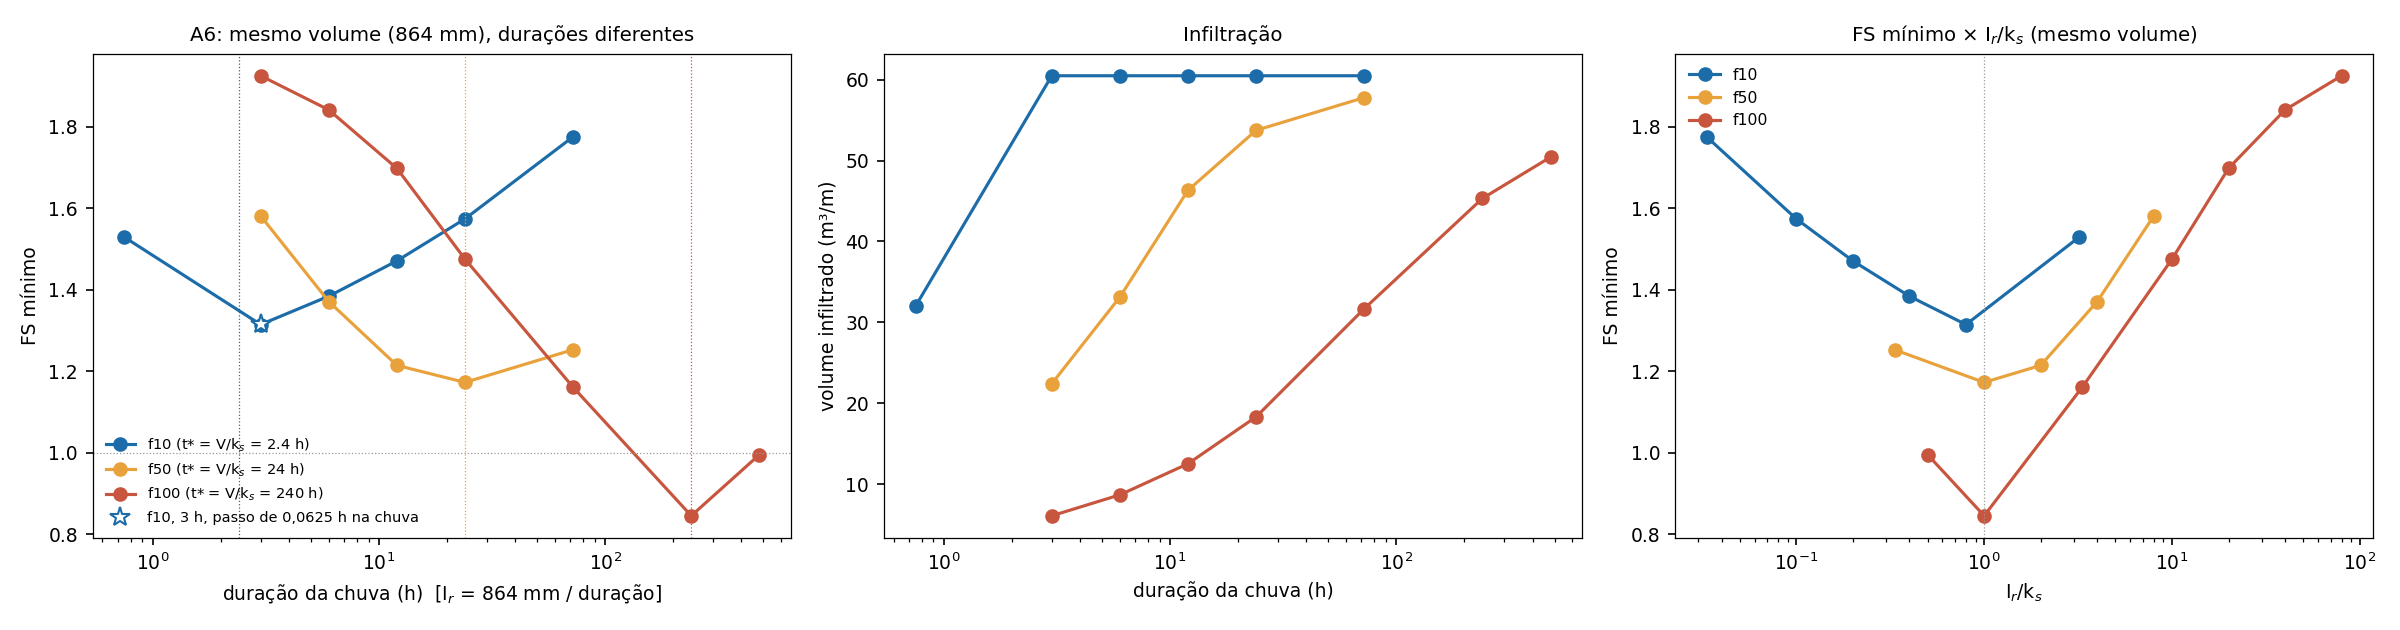
\includegraphics[width=\textwidth]{figuras/contra_A6_volume.png}
\caption{A6: FS m\'inimo e volume infiltrado em fun\c{c}\~ao da dura\c{c}\~ao (pontilhado vertical: $t^*=V/k_s$) e FS
m\'inimo em fun\c{c}\~ao de $I_r/k_s$, com o mesmo volume de chuva (864~mm); estrela: $f_{10}$ com 3~h e passo de
tempo de 0,0625~h.}\label{fig:disc_A6}
\end{figure}

\textbf{Conclus\~ao.} Lidos por solo, os resultados confirmam o sentido do argumento nas faixas de dura\c{c}\~ao
testadas inicialmente (3 a 72~h): no $f_{100}$ o FS m\'inimo cai com a dura\c{c}\~ao, no $f_{10}$ sobe (linearmente com o
logaritmo da dura\c{c}\~ao, mais do que com a dura\c{c}\~ao: $R^2=0{,}985$ contra 0,917) e no $f_{50}$ tem um m\'inimo em
24~h. As dura\c{c}\~oes acrescentadas mostram que os tr\^es s\~ao o mesmo comportamento, visto em janelas diferentes de
uma curva com m\'inimo perto de $I_r=k_s$, isto \'e, da dura\c{c}\~ao $t^*=V/k_s$ (Fig.~\ref{fig:disc_A6}, \`a direita):
o $f_{10}$ volta a subir abaixo de $t^*=2{,}4$~h (1,53 com 0,75~h, contra 1,31 com 3~h; com o passo de tempo 4 vezes
menor a chuva de 3~h d\'a 1,317, contra 1,315, diferen\c{c}a menor que a resolu\c{c}\~ao de 0,01) e o $f_{100}$ tem o
menor FS com 240~h (0,85, contra 1,16 com 72~h e 1,00 com 480~h). Com dois vizinhos por solo, os dados cercam o
m\'inimo sem localiz\'a-lo com precis\~ao: entre $I_r/k_s=0{,}4$ e 3,2 no $f_{10}$, 0,33 e 2 no $f_{50}$ e 0,5 e 3,3 no
$f_{100}$. Acima de $k_s$ a superf\'icie alaga e parte da chuva escorre (no $f_{10}$ com 0,75~h infiltram 53\%; no
$f_{100}$ com 24~h, 30\%). Nas chuvas longas do $f_{100}$ tamb\'em h\'a escoamento, depois que a superf\'icie alaga (com
240~h infiltram 75\%, com 480~h 83\%), mas com 480~h a \'agua drena enquanto chega: \`as 480~h s\'o 70\% dos v\'ertices
t\^em $p_w>-2$~kPa, contra 100\% \`as 240~h, e o FS fica maior. O valor do m\'inimo cai quando $k_s$ diminui (1,31,
1,17 e 0,85), e s\'o o $f_{100}$ rompe com esse volume: com 240~h o FS chega a 1 \`as 196~h e, \`as 240~h, o talude est\'a
saturado at\'e a superf\'icie ($p_w\ge0$ em todos os v\'ertices), no patamar 0,84--0,85; com 480~h o FS s\'o chega a 1
\`as 475~h e termina em 0,996, equil\'ibrio limite com a resolu\c{c}\~ao de 0,01. Para um mesmo volume, a chuva mais
perigosa \'e a de intensidade pr\'oxima de $k_s$, e a dura\c{c}\~ao cr\'itica cresce com $1/k_s$.

%----------------------------------------------------------------------
\subsection{Resumo}

\begin{table}[h!]
\centering\small
\caption{Resumo da discuss\~ao dos contraexemplos.}\label{tab:disc_resumo}
\begin{tabular}{p{0.7cm}p{4.3cm}p{9.8cm}}
\toprule
item & argumento & conclus\~ao\\
\midrule
A1 & com FS $\le1$, o que importa \'e se o FS chega a 1 a partir de uma intensidade &
procede; todos os modelos t\^em intensidade cr\'itica, mas com FS $\le1{,}01$ ela \'e $\approx26$~mm/h no modelo completo
com $\psi=0$, 31~mm/h com $\psi=\phi'$ e 48~mm/h no modelo do artigo, que superestima em 55 a 86\% a chuva que rompe o
talude e atrasa a ruptura em 2 a 10~h; a dilat\^ancia n\~ao decide se h\'a intensidade cr\'itica, mas a desloca em cerca
de 20\% e decide o que acontece depois\\
A2 & o ar retido reduz a resist\^encia; FS $=1{,}01$ pode ser ruptura numa malha mais fina &
procede, com duas ressalvas: no modelo toda a zona n\~ao saturada entre a frente e o NA fica pressurizada, e a
suc\c{c}\~ao n\~ao cai (sobe $p_w$); refinando a malha o FS m\'inimo cai 0,003 por refinamento (1,015 a 1,009), sem
convergir: ruptura iminente\\
A3 & a anisotropia importa; o pior caso seria o ortogonal \`a face &
procede quanto \`a import\^ancia, mas o pior caso depende da chuva: pela intensidade cr\'itica nenhuma orienta\c{c}\~ao
\'e pior que a isotr\'opica (51~mm/h; 79 com $k_1$ normal \`a face; horizontal n\~ao rompe); nas chuvas fortes $k_1$
paralelo \`a face antecipa a ruptura (11 contra 20~h com 90~mm/h), e com 180--360~mm/h o ortogonal fica quase t\~ao
desfavor\'avel quanto o paralelo\\
A4 & sem limite, o FS inicial \'e alto e a queda dr\'astica: suc\c{c}\~ao baixa d\'a falsa seguran\c{c}a? &
a queda procede, a falsa seguran\c{c}a n\~ao: limitar a suc\c{c}\~ao d\'a FS m\'inimo menor (conservador); ela vem de confiar
no FS inicial com suc\c{c}\~ao alta e $\chi=1$; com $\chi=S_e$ o ganho inicial e a queda sem limite caem pela metade\\
A5 & a n\~ao linearidade tem pouco impacto &
procede (erro da reta de 0,03 a 0,07); as inclina\c{c}\~oes da Fig.~9 s\~ao 17 a 28\% maiores que as calculadas; a
geometria n\~ao \'e secund\'aria: o \^angulo sozinho leva \`a ruptura ($\alpha\approx60^\circ$ no $f_{10}$ e no
$f_{50}$)\\
A6 & com o mesmo volume, a dura\c{c}\~ao pesa e o efeito depende do solo &
procede, e os tr\^es comportamentos s\~ao janelas de uma curva com m\'inimo perto de $I_r=k_s$ ($t^*=V/k_s$), compat\'ivel
com os tr\^es solos; o m\'inimo cai quando $k_s$ diminui (1,31, 1,17 e 0,85) e s\'o o $f_{100}$ rompe com esse volume\\
\bottomrule
\end{tabular}
\end{table}

Com o crit\'erio FS $\le1$, os modelos devem ser comparados pela intensidade cr\'itica e pelo instante da ruptura, e
n\~ao pelo FS m\'inimo. Nessa compara\c{c}\~ao, a percola\c{c}\~ao desacoplada com ar passivo superestima a chuva que rompe
o talude e atrasa a ruptura (A1); o ar ativo reduz a margem at\'e a ruptura em 0,08 a 0,22, e o caso mais desfavor\'avel
do A2 fica no equil\'ibrio limite (A2); a isotropia n\~ao altera a intensidade cr\'itica, mas atrasa a ruptura nas chuvas
fortes em rela\c{c}\~ao a $k_1$ paralelo ou normal \`a face (A3); o limite da suc\c{c}\~ao inicial \'e conservador, e o risco
de falsa seguran\c{c}a est\'a no FS inicial calculado com suc\c{c}\~ao alta e $\chi=1$ (A4); a geometria e a dura\c{c}\~ao
da chuva, em rela\c{c}\~ao a $V/k_s$, n\~ao s\~ao secund\'arias (A5, A6).


\end{document}
